\documentclass{article} % For LaTeX2e
\usepackage{icml2016}
\usepackage{times}
\usepackage{hyperref}
\usepackage{changes}
\usepackage{url}
\usepackage{amssymb}
\usepackage{enumitem}
\setcounter{tocdepth}{3}
\usepackage{graphicx}
\usepackage{color}
\usepackage{hyperref}
\usepackage{amsmath}
\usepackage{amssymb}
\usepackage{amsthm}
\usepackage{graphicx}
\usepackage{tabularx}
\usepackage{fancyvrb}
\usepackage{comment}
\usepackage{algorithm}
\usepackage{algorithmic}
\usepackage{mathtools}
\usepackage{float}
\usepackage{wrapfig}

\renewcommand{\algorithmicrequire}{\textbf{Input:}}
\renewcommand{\algorithmicensure}{\textbf{Output:}}

\newcommand{\abs}[1]{\lvert#1\rvert}
\newcommand{\norm}[1]{\lVert#1\rVert}
\newcommand{\RR}{\mathbb{R}}
\newcommand{\Nat}{\mathbb{N}}
\newcommand{\CC}{\mathbb{C}}
\DeclareMathOperator*{\argmin}{arg\,min}
\DeclareMathOperator*{\argmax}{arg\,max}

\theoremstyle{definition}
\newtheorem{conjecture}{Conjecture}
\newtheorem{example}{Example}
\newtheorem{theorem}{Theorem}
\newtheorem{lemma}[theorem]{Lemma}
\newtheorem{definition}[theorem]{Definition}
\newtheorem{proposition}{Proposition}
\newtheorem{corollary}{Corollary}

\newcommand{\defeq}{\vcentcolon=}
\newcommand{\eqdef}{=\vcentcolon}

\setlist{nolistsep}
\setlength{\itemsep}{0pt}

\icmltitlerunning{Collapsed Variational Inference for Sum-Product Networks}

\begin{document} 

\twocolumn[
\icmltitle{Collapsed Variational Inference for Sum-Product Networks}

% It is OKAY to include author information, even for blind
% submissions: the style file will automatically remove it for you
% unless you've provided the [accepted] option to the icml2014
% package.
\icmlauthor{Han Zhao$^\dagger$}{han.zhao@cs.cmu.edu}
\icmlauthor{Brandon Amos$^\dagger$}{bamos@cs.cmu.edu}
\icmlauthor{Tameem Adel$^\S$}{ T.M.A.A.Hesham@uva.nl}
\icmladdress{$^\dagger$School of Computer Science, Carnegie Mellon University, Pittsburgh, PA, USA \\
$^\S$Machine Learning Lab, University of Amsterdam, Amsterdam, the Netherlands}

\icmlkeywords{Sum-Product Network, Collapsed Variational Inference}

\vskip 0.3in
]

\begin{abstract}
Sum-Product Networks (SPNs) are probabilistic inference machines that admit exact inference in linear time in the size of the network. Existing parameter learning approaches for SPNs are largely based on the maximum likelihood principle and hence are subject to overfitting when the data available is small.
Vanilla variational inference for sum-product networks is computationally intractable due to the large number of latent variables per instance. In this work, we propose a novel collapsed variational inference algorithm for SPNs that is computationally efficient, easy to implement and at the same time allows us to incorporate prior information into the optimization formulation. Extensive experiments show a significant improvement in accuracy. 
\end{abstract}

\section{Introduction}
\label{sec:intro}
%Probabilistic graphical models including Bayesian networks and Markov networks are powerful tools for modeling complex distributions and reasoning under uncertainty. However, a compact representation in probabilistic graphical models does not lead to tractable inference. It is known that exact inference in probabilistic graphical models is \texttt{\#P} complete due to its connection to weighted model counting~\cite{gomes2008model}; even approximate inference with $\epsilon$-guarantee is NP-hard~\cite{roth1996hardness}. As a step towards tractable inference, Sum-Product Networks (SPNs) have been proposed as tractable deep models for exact probabilistic inference~\cite{poon2011sum}. Probabilistic inferences, including joint inference, marginal inference and conditional inference, can be performed exactly in SPNs in linear time with respect to the network size. Due to their tractability and flexibility, SPNs have been widely applied in various fields, e.g., image completion~\cite{poon2011sum,dennis2012learning}, activity modeling~\cite{amer2012sum}, speech modeling~\cite{peharz2014modeling}, language modeling~\cite{cheng2014spnlm} and density estimation~\cite{gens2013learning,rooshenas2014learning}, to name a few. 

Parameter learning and structure learning are two important research problems in Sum-product networks (SPNs)~\cite{gens2013learning,zhao2015unifying,gens2012discriminative}. The structure learning problem concerns automatic construction of the network structure by exploiting probabilistic independences among variables of interest from the data. Given an SPN with fixed structure, existing parameter learning algorithms focus on learning SPNs based on the maximum likelihood principle by viewing them as generative probabilistic models. It has been recently shown that the optimization formulation based on the maximum likelihood principle can be equivalently transformed into a difference of convex programs, and efficient algorithms like the concave-convex procedure have been designed to tackle this problem~\cite{zhao2015unifying}. 

Since those algorithms maximize the likelihood of the data, they are subject to overfitting and it is hard to incorporate prior information into the design of the algorithm. In this work we propose a novel Bayesian learning algorithm that is robust to overfitting and can be naturally extended into stochastic setting to scale to large data sets. To the best of our knowledge, this is the first general Bayesian approach to learn the parameters of SPNs in both batch and stochastic settings. Bayesian inference of SPNs is challenging, mostly due to the vast amount of local latent variables and their intricate connections. Unlike traditional mixture models, e.g., LDA~\cite{blei2003latent}, Gaussian mixture model, etc, where the number of local latent variables scales linearly as the number of observations, the number of local latent variables in SPNs is linearly proportional to the size of the network, often around thousands to millions, for each observable instance. Furthermore, once given the observation, those latent variables are coupled with each other in a complicated manner, which makes Bayesian learning even harder in SPNs. As we will see later, exact Bayesian learning in the setting of SPNs is intractable due to the exponential growth of the number of mixture components in the posterior distribution.

The vanilla variational inference approach and Gibbs sampling method are not feasible for SPNs due to the large amount of local latent variables per observation. To deal with these problems, our approach works in a collapsed space and approximates the exact posterior with variational distributions. However, different from traditional collapsed variational approach in the literature that marginalize out global latent variables~\cite{teh2006collapsed,teh2007collapsed} in order to spread out the interactions among many local latent variables, here we consider a complementary approach. Instead of marginalizing out the global latent variables, we \emph{marginalize out the local latent variables} and maintain a variational posterior distribution directly on the global latent variables, i.e., the model parameters. The posterior mean over the variational distribution of model parameters can then be used as a Bayesian estimator as desired. At the first glance, marginalizing out the local latent variables of the observable instances in general graphical models seems to be a bad idea because of two reasons. First, by marginalizing out local latent variables we incur a computation that is exponential in the tree-width of the graph~\cite{wainwright2008graphical}. Except for graphical models with special structures, for examples, LDA, Gaussian mixture models, thin junction trees, etc, such exact computation is by itself intractable. Second, the marginalization will in general invalidate the conjugacy between the prior distribution and the joint distribution over global and local latent variables, which further makes the expectation over variational posterior intractable. Fortunately, as we will show later, the ability of SPNs to model context-specific independence helps to solve the first problem and by using a change of variable transformation our approach handles the second problem efficiently. We call our approach CVB-SPN. To show the validity of CVB-SPN, we conduct extensive experiments and compare it with methods based on the maximum likelihood principle in both batch and stochastic settings.

\section{Background}
\label{sec:background}
\subsection{Sum-Product Networks}
A sum-product network (SPN) is a graphical representation of a joint probability distribution over a set of random variables $\mathbf{X} = \{X_1, \ldots, X_n\}$. It is a rooted directed acyclic graph where the interior nodes are sums or products and the leaves are univariate distributions over $X_i$. Edges emanating from sum nodes are parameterized with positive weights. Each node in SPNs encodes an unnormalized marginal distribution over $\mathbf{X}$. Let $\mathbf{x}$ be a joint instantiation of the random vector $\mathbf{X}$ and let $V_k(\mathbf{x}|\mathbf{w})$ be the value associated with node $k$ when the input to the network is $\mathbf{x}$ with network weights set to be $\mathbf{w}$. The values for each node in an SPN can computed recursively as follows:
\begin{equation}
\small
\label{eq:network-eval}
V_k(\mathbf{x}|\mathbf{w}) = 
\begin{cases}
p(X_i = \mathbf{x}_i) & \text{$k$ is a leaf node over $X_i$} \\
\prod_{j \in Ch(k)} V_j(\mathbf{x}|\mathbf{w}) & \text{$k$ is a product node} \\
\sum_{j\in Ch(k)} w_{kj} V_j(\mathbf{x}|\mathbf{w}) & \text{$k$ is a sum node}
\end{cases} 
\end{equation}
where $Ch(k)$ is the children list of node $k$ in the graph and $w_{kj}$ is the edge weight associated with sum node $k$ to its child node $j$.
The joint distribution encoded by an SPN is then defined by the graphical structure and the weights. The probability/density of a joint assignment $\mathbf{X}=\mathbf{x}$ is proportional to the value at the root of the SPN with input $\mathbf{x}$ divided by a normalization constant $V_{root}(\mathbf{1}|\mathbf{w})$:
\begin{equation}
\label{eq:joint-prob}
p(\mathbf{x}) = \frac{V_{root}(\mathbf{x}|\mathbf{w})}{V_{root}(\mathbf{1}|\mathbf{w})}
\end{equation}
where the normalization constant $V_{root}(\mathbf{1}|\mathbf{w})$ is obtained by setting all the values of leaf nodes to be 1. Intuitively, setting all the leaf nodes to be 1 corresponds to integrating/marginalizing out the random vector $\mathbf{X}$, which will ensure Eq.~\ref{eq:joint-prob} defines a proper probability distribution for both discrete and continuous random variables. Eq.~\ref{eq:joint-prob} can also be used to compute the marginal probability of a partial assignment $\mathbf{Y}=\mathbf{y}$: simply set the value of leaf nodes $n$ whose corresponding random variable is not in $\mathbf{Y}$ to be 1 and the value of other leaf nodes based on the assignment $\mathbf{Y} = \mathbf{y}$.  Intuitively, this corresponds to integrating out variables outside of the partial assignment. Conditional probabilities can also be computed by evaluating two partial assignments:
\begin{equation*}
p(\mathbf{Y} =\mathbf{y}|\mathbf{Z}=\mathbf{z}) = \frac{p(\mathbf{Y}=\mathbf{y},\mathbf{Z}=\mathbf{z})}{p(\mathbf{Z}=\mathbf{z})} 
= \frac{V_{root}(\mathbf{y},\mathbf{z}|\mathbf{w})}{V_{root}(\mathbf{z}|\mathbf{w})}
\end{equation*}
Since joint, marginal and inference queries can all be computed by two network passes, exact inference takes linear time with respect to the network size. For the completeness of the discussion, we also list the following definitions given by~\citet{poon2011sum}:
\begin{definition}[scope]
The scope of a node $n$ is the set of all variables that appear in the leaf univariate distributions of the sub-SPN rooted at $n$.
\end{definition}
\begin{definition}[completeness]
An SPN is complete when each sum node has children with identical scope.
\end{definition}
\begin{definition}[decomposability] 
An SPN is decomposable when each product node has children with disjoint scopes.
\end{definition}
Without loss of generality, in this paper we focus our attention on the case where all the random variables $X_i$ are boolean variables. However, direct extension to the continuous case is not hard, one can simply replace each univariate distribution at the leaves of the graph with desired continuous distributions. 

\subsection{SPNs as Mixture Models}
It has been recently shown that any complete and decomposable SPN $\mathcal{S}$ over $\mathbf{X} =\{X_1,\ldots, X_n\}$ is equivalent to a Bayes network with $O(n|\mathcal{S}|)$ size~\cite{zhao2015spnbn}. The insight behind the construction process is that each internal sum node in $\mathcal{S}$ corresponds to a latent variable in the constructed Bayes net and the Bayes network will be a bipartite graph with one layer of latent variables pointing to one layer of observable variables $\mathbf{X}$. Equivalently, this shows that the SPN $\mathcal{S}$ can be interpreted as a graphical model where the number of latent variables is $O(|\mathcal{S}|)$. Although the Bayes network perspective of SPNs provides an interesting connection between the two models, we can hardly work on the Bayes net in practice due to the large number of latent variables ($O(|\mathcal{S}|)$) in the graph. In fact, a naive expansion of such Bayes net will lead to a mixture model with $O(2^{|\mathcal{S}|})$ components which is not feasible to work with directly. 

Another result is that an SPN, as a directed acyclic graph, can be decomposed into a sum of induced trees~\cite{zhao2015unifying}. The definition of induced SPNs is as follows:
\begin{definition}[Induced SPN]
\label{def:treespn}
Given a complete and decomposable SPN $\mathcal{S}$ over $\mathbf{X}= \{X_1,\ldots, X_n\}$, $\mathcal{T}$ is called an \emph{induced SPN} from $\mathcal{S}$ if 
\begin{enumerate}
	\item 	$Root(\mathcal{S})\in\mathcal{T}_V$.
	\item 	If $v\in\mathcal{T}_V$ is a sum node, then exactly one child of $v$ in $\mathcal{S}$ is in $\mathcal{T}_V$, with the corresponding edge in $\mathcal{T}_E$.
	\item 	If $v\in\mathcal{T}_V$ is a product node, then all the children of $v$ in $\mathcal{S}$ are in $\mathcal{T}_V$, with the corresponding edges in $\mathcal{T}_E$.
\end{enumerate}
where in the definition above $\mathcal{T}_V$ is the node set of $\mathcal{T}$ and $\mathcal{T}_E$ is the edge set of $\mathcal{T}$.
\end{definition}
\begin{figure}[htb]
\centering
	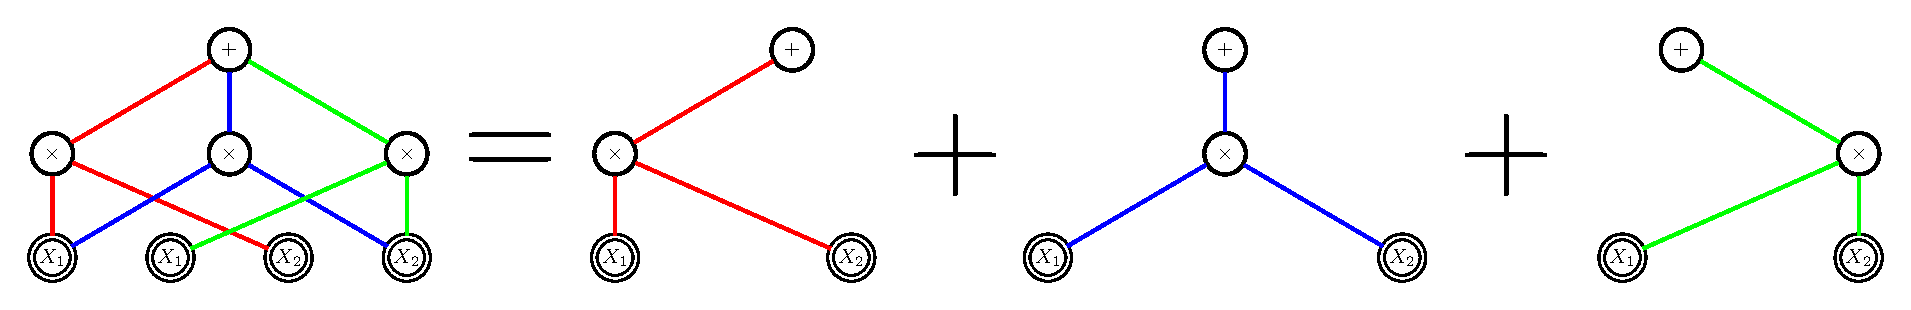
\includegraphics[width=\linewidth]{figures/spntrees.pdf}
\caption{Induced tree decomposition of a complete and decomposable SPN into a mixture model where each component is characterized by a product of univariate distributions over $X_1$ and $X_2$.}
\label{fig:spntrees}
\end{figure}
It has been shown that every induced SPN from a complete and decomposable SPN must form a tree~\cite{zhao2015unifying}. A key result based on the notion of induced trees that exhibits the distribution modeled by SPNs is~\cite{zhao2015unifying}:
\begin{theorem}
\label{thm:polynomial}
Let $\tau_\mathcal{S} = V_{root}(\mathbf{1}|\mathbf{1})$, then $V_{root}(\mathbf{x}|\mathbf{w}) = \sum_{t=1}^{\tau_\mathcal{S}}\prod_{(k, j)\in\mathcal{T}_{tE}}w_{kj}\prod_{i=1}^n p_t(X_i = \mathbf{x}_i)$, where $\mathcal{T}_t$ is the $t$th unique induced tree of $\mathcal{S}$ and $p_t(X_i)$ is a univariate distribution over $X_i$ in $\mathcal{T}_t$ as a leaf node.
\end{theorem}
Fig.~\ref{fig:spntrees} gives an illustrative example of Thm.~\ref{thm:polynomial}. Thm.~\ref{thm:polynomial} characterizes both the number of components and the form of each component in the mixture model. Compared with a naive expansion of the Bayes net that leads to a mixture model with $O(2^{|\mathcal{S}|})$ components, the mixture model given in Thm.~\ref{thm:polynomial} is more compact. In the next section we will develop our CVB-SPN method based on Thm.~\ref{thm:polynomial}.

\subsection{Variational Bayes Inference}
Standard variational Bayes inference is an optimization-based approach to approximate the full posterior distribution of both the global and local latent variables of a Bayesian model~\cite{jordan1999introduction}. It approximates the full posterior distribution by constructing and maximizing an evidence lower bound (ELBO) of the log marginal likelihood function $\log p(\mathbf{x})$. Equivalently, one can minimize the Kullback-Leibler divergence between the true posterior distribution and the variational posterior distribution. To review, let $\Theta = \{\mathbf{H}, \mathbf{W}\}$ represent the set of latent variables in a Bayesian model (including both the global and local latent variables) and let $\mathbf{X}$ represent the data. The joint probability distribution of $\Theta$ and $\mathbf{X}$ is $p(\mathbf{X}, \Theta~|~\pmb\alpha)$ where $\pmb\alpha$ is the set of hyperparameters of the model. Standard variational inference approximates the true posterior $p(\Theta~|~\mathbf{X}, \pmb\alpha)$ with a variational  distribution $q(\Theta~|~\pmb\beta)$ with a set of variational parameters $\pmb\beta$. This reduces an inference problem into an optimization problem in which the objective function is given by the ELBO $\mathcal{L}(\pmb\beta)$:
\begin{equation*}
\log p(\mathbf{x}|\pmb\alpha) \geq \mathbb{E}_{q}[\log p(\mathbf{x}, \Theta|\pmb\alpha)] + \mathbb{H}[q(\Theta|\pmb\beta)] =\vcentcolon \mathcal{L}(\pmb\beta)
\end{equation*}
where $\mathbb{H}[\cdot]$ is the entropy functional. The variational distribution $q(\Theta~|~\pmb\beta)$ is assumed to be fully factorized with each variational parameter $\beta_i$ governing one latent variable $\theta_i$. The set of variational parameters are then optimized to maximize the ELBO until convergence and the optimal variational posterior will be used as a surrogate distribution to the true posterior distribution $p(\Theta~|~\mathbf{X}, \pmb\alpha)$. It is worth noting that in the standard variational Bayes inference the number of variational parameters to be optimized is linearly proportional to the number of latent variables, including both the global and local latent variables.

\section{Collapsed Variational Bayesian Inference for SPNs}
\subsection{Motivation}
A graphical model representation of sum-product networks is shown in Fig.~\ref{fig:pgmspn}. In this section we derive a novel Bayesian inference algorithm for sum-product networks, which we call as CVB-SPN. Standard variational inference methods are not computationally feasible for SPNs due to the large number of local latent variables for each training instance, as shown in Fig.~\ref{fig:pgmspn}. Let $\mathbf{W}$ denote the set of global latent variables (model parameters) and $\mathbf{H}_d$ denote the set of local latent variables, where $d$ indexes over the training instances. In standard variational inference approach we need to maintain a set of variational parameters over all the latent variables, i.e., $\mathbf{W}$ and $\{\mathbf{H}_d\}_{d=1}^D$. For mixture models such as LDA or GMM, $\mathbf{H}_d$ corresponds to the topic assignment of the $d$th word and mixture component assignment of $d$th instance. In those models, each observable instance corresponds to only one local latent variable. However,
in the case of SPNs, the number of local latent variables is exactly the number of internal sum nodes in the network, which is linearly proportional to the size of the network, $|\mathcal{S}|$. Together with the global latent variables, this leads to a total number of $O(D|\mathcal{S}| + |\mathcal{S}|)$ variational parameters to be maintained in the vanilla variational inference approach. As we will see in the experiments, this is prohibitively expensive for typical sizes of SPNs that range from tens of thousands to millions. 

To deal with the expensive computation and storage in standard variational inference approach for SPNs, we develop CVB-SPN, a collapsed variational algorithm, which instead of assuming independence among the local latent variables, models the dependence among them in an exact fashion. More specifically, we marginalize all the local latent variables out of the joint posterior distribution and maintain a posterior distribution over the global latent variables directly. On the other hand, we still assume that the global variables (model parameters) are mutually independent. Note this basic assumption made in CVB-SPN is different from typical collapsed variational approaches developed for LDA and HDP~\cite{teh2006collapsed,teh2007collapsed}, where global latent variables are integrated out and local latent variables are assumed to be mutually independent. 
\begin{figure}[htb]
\centering
	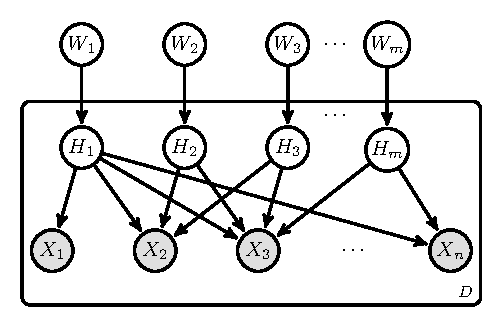
\includegraphics[scale=0.8]{figures/spntemplate.pdf}
\caption{Graphical model representation of SPN $\mathcal{S}$. The box is plate that represents the number of replicates, where $D$ is the number of training instances. $m= O(|\mathcal{S}|)$ corresponds to the number of sum nodes and $n$ is the number of observable random variables in $\mathcal{S}$.}
\label{fig:pgmspn}
\end{figure}
Intuitively, this is not an unreasonable assumption to make since compared with local latent variables, the global latent variables in Fig.~\ref{fig:pgmspn} are more away from the influences of observations of $\mathbf{X}$ and they are mutually independent at the first place if there is no observation of $\mathbf{X}$. Besides the computational consideration, another motivation for us to collapse out the local latent variables is that  there is no specific statistical interpretation associated with the local latent variables that is useful in practice. Unlike other mixture models such as LDA or GMM, where the value of local latent variables correspond to the topic assignment of words or the cluster assignment of instances, the sum nodes in SPNs do not share specific statistical interpretations that are useful in real-world applications. 

As a result, CVB-SPN models the marginal posterior distribution over global latent variables only and hence the number of variational parameters to be optimized is $O(|\mathcal{S}|)$ compared with $O(D|\mathcal{S}|)$ in the standard case. As usual, the optimal variational posterior over global latent variables can be used to induce a Bayesian estimator, e.g., the posterior mean, of the model parameters. With less assumptions about the independency among random variables and less variational variables to be optimized, CVB-SPN faces two questions: first, the cost of exact marginalization over local latent variables and the non-conjugacy between the prior distribution and the likelihood function introduced by the marginalization.    The first problem is elegantly handled by the property of SPN that exact inference over $\mathbf{X}$ is always tractable due to its ability of modeling context-specific independence~\cite{boutilier1996context}. In what follows we proceed to derive the CVB-SPN algorithm that efficiently solves the second problem.

\subsection{Collapsed Variational Inference}
Throughout the derivation we will assume that the weights $w_{kj}$ associated with a sum node $k$ is locally normalized, i.e., $\sum_{j\in Ch(k)}w_{kj} = 1, \forall k$. This can be achieved by a bottom-up pass of the network in $O(|\mathcal{S}|)$ without changing the joint probability distribution over $\mathbf{X}$, see~\citet{peharz2015foundations} and~\citet{zhao2015spnbn} for more details about the algorithm to do this. For SPNs with locally normalized weights $\mathbf{w}$, it can be verified that $V_{root}(\mathbf{1}|\mathbf{w}) = 1$, hence the marginal likelihood function $p(\mathbf{x}|\mathbf{w})$ that marginalizes out local latent variables $\mathbf{h}$ is given by $V_{root}(\mathbf{x}|\mathbf{w})$. 

Since the weights associated with each sum node $k$ are locally normalized, we can interpret each sum node to be a multinomial random variable where the number of values taken by this multinomial variable is equal to the number of children of the sum node. It follows that we can specify a Dirichlet prior $Dir(w_k|\alpha_k)$ for each sum node $k$. For the convenience of notation we assume the prior $Dir(w_k|\alpha_k)$ to be a symmetric Dirichlet, i.e., $Dir(w_k|\alpha_k)\defeq Dir(w_k|\alpha_k\mathbf{1})$\footnote{In practice this is not a constraint as one can choose any Dirichlet prior and the analysis follows the same.}. From Fig.~\ref{fig:pgmspn} it can be checked that all the $w_k$ are $d$-separated without observation $\mathbf{x}$, hence a prior distribution over all the weights can be factorized as:
\begin{equation}
p(\mathbf{w}|\pmb\alpha) = \prod_{k=1}^m p(w_k|\alpha_k) = \prod_{k=1}^m Dir(w_k|\alpha_k)
\end{equation}
Based on Thm.~\ref{thm:polynomial}, the true posterior distribution after a sequence of observations $\{\mathbf{x}_d\}_{d=1}^D$ is:
\begin{align}
& p(\mathbf{w}|\{\mathbf{x}_d\}_{d=1}^D, \pmb\alpha) \propto p(\mathbf{w}|\pmb\alpha)\prod_{d=1}^D V_{root}(\mathbf{x}_d|\mathbf{w}) \nonumber\\
= & \prod_{k=1}^m Dir(w_k|\alpha_k)\prod_{d=1}^D \sum_{t=1}^{\tau_\mathcal{S}}\prod_{(k, j)\in\mathcal{T}_{tE}}w_{kj}\prod_{i=1}^n p_t(x_{di})
\label{equ:posterior}
\end{align}
For discrete SPNs the leaf univariate distributions are simply point mass distributions, i.e., indicator variables. For continuous distributions such as Gaussians, we also need to specify the priors for the parameters of those leaf distributions but the analysis goes the same as the discrete case. Eq.~\ref{equ:posterior} points out that the true posterior distribution of the model parameters is a mixture of product of Dirichlets where the number of components scales as $\tau_\mathcal{S}^D$ and each component is a product of $m$ Dirichlets, one for each sum node. This is intractable to compute exactly, hence we resort to collapsed variational inference method. To simplify the notation, we will assume that there is only one instance in the data set, i.e., $D = 1$. Extension of the following derivation to multiple training instances is straightforward. Consider the log marginal probability over observable variables that upper bounds the ELBO $\mathcal{L}(\pmb\beta)$:
\begin{align}
\log p(\mathbf{x}|\pmb\alpha) & \geq \mathbb{E}_{q(\mathbf{w})}[\log p(\mathbf{x}, \mathbf{w}| \pmb\alpha)] + \mathbb{H}[q(\mathbf{w}|\pmb\beta)] \\
& = \mathbb{E}_{q(\mathbf{w})}[\log\sum_{\mathbf{h}} p(\mathbf{x}, \mathbf{h}, \mathbf{w}| \pmb\alpha)] + \mathbb{H}[q(\mathbf{w}|\pmb\beta)] \nonumber
\label{equ:elbo}
\end{align}
where $q(\mathbf{w}|\pmb\beta) = \prod_{k=1}^m Dir(w_k|\beta_k)$ is the factorized variational distribution over $\mathbf{w}$ to approximate the true marginal posterior distribution $p(\mathbf{w}|\mathbf{x}, \pmb\alpha) = \sum_{\mathbf{h}}p(\mathbf{w}, \mathbf{h}|\mathbf{x},\pmb\alpha)$. We argue that $\mathcal{L}(\pmb\beta)$ gives us a better lower bound to optimize than the one given by the standard variational inference. To see this, let $\widehat{\mathcal{L}}(\pmb\beta)$ be the ELBO given by standard variational inference, i.e., 
$$\widehat{\mathcal{L}}(\pmb\beta) = \mathbf{E}_{q(\mathbf{w})q(\mathbf{h})}[\log p(\mathbf{x}, \mathbf{w}, \mathbf{h}|\pmb\alpha)] + \mathbb{H}[q(\mathbf{w})q(\mathbf{h})]$$
we have:
\begin{align*}
\small
\mathcal{L}(\pmb\beta) &= \mathbb{E}_{q(\mathbf{w})}[\log p(\mathbf{x}, \mathbf{w}|\pmb\alpha)] + \mathbb{H}[q(\mathbf{w})] \nonumber \\
& = \mathbb{E}_{q(\mathbf{w})}\left[\mathbb{E}_{p(\mathbf{h}|\mathbf{w}, \mathbf{x}, \mathbf{\alpha})}[\log \frac{p(\mathbf{h}, \mathbf{w}, \mathbf{x}| \mathbf{\alpha})}{p(\mathbf{h}|\mathbf{w}, \mathbf{x}, \mathbf{\alpha})}]\right] + \mathbb{H}[q(\mathbf{w})] \nonumber\\
& = \max_{q(\mathbf{h}|\mathbf{w})}\mathbb{E}_{q(\mathbf{w})}\left[\mathbb{E}_{q(\mathbf{h}|\mathbf{w})}[\log\frac{p(\mathbf{h}, \mathbf{w}, \mathbf{x}| \mathbf{\alpha})}{q(\mathbf{h}|\mathbf{w})}]\right] + \mathbb{H}[q(\mathbf{w})] \\
&\geq \max_{q(\mathbf{h})}\mathbb{E}_{q(\mathbf{w})}\left[\mathbb{E}_{q(\mathbf{h})}[\log\frac{p(\mathbf{h}, \mathbf{w}, \mathbf{x}| \mathbf{\alpha})}{q(\mathbf{h})}]\right] + \mathbb{H}[q(\mathbf{w})] \\
& \geq \mathbb{E}_{q(\mathbf{w})q(\mathbf{h})}[\log p(\mathbf{x}, \mathbf{w}, \mathbf{h}|\pmb\alpha)] + \mathbb{H}[q(\mathbf{w})q(\mathbf{h})] \nonumber\\
& = \widehat{\mathcal{L}}(\pmb\beta)
\end{align*}
where the maximization over $q(\mathbf{h}|\mathbf{w})$ is free of constraint hence the optimal posterior is given by the true conditional posterior $q^*(\mathbf{h}|\mathbf{w}) = p(\mathbf{h}|\mathbf{w}, \mathbf{x}, \pmb\alpha)$, while the maximization over $q(\mathbf{h})$ needs to satisfy the independence assumption made in the standard variational inference, i.e., $q(\mathbf{h}|\mathbf{w}) = q(\mathbf{h})$. Hence the first inequality holds. Combine the inequality above with Eq.~\ref{equ:posterior}, we have
\begin{equation}
\log p(\mathbf{x}|\pmb\alpha)\geq \mathcal{L}(\pmb\beta)\geq \widehat{\mathcal{L}}(\pmb\beta)
\end{equation}
which shows that the ELBO given by the collapsed variational inference is a better lower bound than the one given by standard variational inference. This conclusion is also consistent with the one obtained in collapsed variational inference for LDA and HDP~\cite{teh2006collapsed,teh2007collapsed} where the authors collapsed out the global latent variables instead of the local latent variables. 

It is also straightforward to verify that the difference between $\log p(\mathbf{x}|\pmb\alpha)$ and $\mathcal{L}(\pmb\beta)$ is given by $\mathbb{KL}(q(\mathbf{w}|\pmb\beta)||p(\mathbf{w}|\mathbf{x},\pmb\alpha))$, i.e., the KL-divergence between the variational marginal posterior and the exact marginal posterior distribution. Substituting $q(\mathbf{w}|\pmb\beta)$ into the KL-divergence objective and simplifying it, we reach the following optimization objective:
\begin{equation}
\underset{\pmb\beta}{\text{minimize}}\quad\mathbb{KL}(q(\mathbf{w}|\pmb\beta) || p(\mathbf{w}|\pmb\alpha)) - \mathbb{E}_{q(\mathbf{w}|\pmb\beta)}[\log p(\mathbf{x}|\mathbf{w})]
\label{equ:primeopt}
\end{equation}
where the first term is a regularization term that penalizes the variational posterior which is too far away from the prior, and the second term is a data-fitting term that requires the variational posterior to have a good fit to the training data set. Due to the factorization assumption of both the prior and the variational posterior distribution, the first term in (\ref{equ:primeopt}) can be efficiently computed. However, the second term does not admit an analytic form. This is because after we marginalize out the local latent variables, $q(\mathbf{w}|\pmb\beta)$ is no longer conjugate to the likelihood function $p(\mathbf{x}|\mathbf{w}) = V_{root}(\mathbf{x}|\mathbf{w})$.

\subsection{Upper Bound by Logarithmic Transformation}
The hardness in the computation of $\mathbb{E}_{q(\mathbf{w}|\pmb\beta)}[\log p(\mathbf{x}|\mathbf{w})]$ makes the direct optimization of (\ref{equ:primeopt}) not feasible in practice. In this section we show how to use a logarithmic transformation trick to develop an upper bound of the objective in (\ref{equ:primeopt}) which leads to the CVB-SPN algorithm that is computationally as efficient as expectation maximization while is robust to overfitting and is flexible to incorporate prior information. 

The key observation here is that the likelihood function of $\mathbf{w}$ is a posynomial function~\cite{boyd2007tutorial}. To see this, as shown in Thm.~\ref{thm:polynomial}, we have $p(\mathbf{x}|\mathbf{w}) = \sum_{t=1}^{\tau_\mathcal{S}}\prod_{(k, j)\in\mathcal{T}_{tE}}w_{kj}\prod_{i=1}^n p_t(X_i = \mathbf{x}_i)$. The product term with respect to $\mathbf{x}$, $\prod_{i=1}^n p_t(X_i = \mathbf{x}_i)$, is guaranteed to be nonnegative and can be treated as a constant w.r.t. $\mathbf{w}$. Hence each component in $p(\mathbf{x}|\mathbf{w})$, in terms of $\mathbf{w}$, is a monomial function with positive multiplicative constant, and it follows that $p(\mathbf{x}|\mathbf{w})$ is a posynomial function of $\mathbf{w}$. A natural implication of this observation is that we can do a change of variable transformation of $\mathbf{w}$ such that $\log p(\mathbf{x}|\mathbf{w})$ becomes a convex function in terms of the transformed variables. More specifically, let $\mathbf{w}' = \log\mathbf{w}$, where $\log(\cdot)$ is taken elementwisely. The log likelihood function, now expressed in terms of $\mathbf{w}'$, is
\begin{align}
\log p(\mathbf{x}|\mathbf{w}) & = \log\left(\sum_{t=1}^{\tau_\mathcal{S}}\prod_{(k, j)\in\mathcal{T}_{tE}}w_{kj}\prod_{i=1}^n p_t(X_i = \mathbf{x}_i)\right) \nonumber\\ 
& = \log\left(\sum_{t=1}^{\tau_\mathcal{S}}\exp\left(c_t + \sum_{(k, j)\in \mathcal{T}_{tE}}w'_{kj}\right)\right) \nonumber\\
& \eqdef \log p(\mathbf{x}|\exp(\mathbf{w}'))
\end{align}
where $c_t$ is defined as $c_t = \log\prod_{i=1}^n p_t(X_i = \mathbf{x}_i)$. For each unique tree $\mathcal{T}_t$, $c_t + \sum_{(k, j)\in \mathcal{T}_{tE}}w'_{kj}$ is an affine function of $\mathbf{w}'$ and note that the log-sum-exp function is convex in its argument, hence it can be readily verified that $\log p(\mathbf{x}|\exp(\mathbf{w}'))$ is convex in $\mathbf{w}'$. Such change of variable trick is frequently applied in the geometric programming literature to transform a non-convex posynomial optimization problem into a convex programming problem, see~\cite{boyd2007tutorial,chiang2005geometric} for more discussions on this topic. 

The convexity of $\log p(\mathbf{x}|\exp(\mathbf{w}'))$ helps us to develop a lower bound of $\mathbb{E}_{q(\mathbf{w}|\pmb\beta)}[\log p(\mathbf{x}|\mathbf{w})]$ that is efficient to compute. Let $q'(\mathbf{w}')$ be the corresponding variational distribution over $\mathbf{w}'$ generated from $q(\mathbf{w})$, we have
\begin{align*}
\mathbb{E}_{q(\mathbf{w})}[\log p(\mathbf{x}|\mathbf{w})] & = \int q(\mathbf{w}) \log p(\mathbf{x}|\mathbf{w})~d\mathbf{w} \\
& = \int q'(\mathbf{w}') \log p(\mathbf{x}|\exp(\mathbf{w}'))~d\mathbf{w}' \\
& \geq \log p(\mathbf{x}|\exp(\mathbb{E}_{q'(\mathbf{w}')}[\mathbf{w}']))
\end{align*}
Note that $q(\mathbf{w}) = \prod_{k=1}^m Dir(w_k | \beta_k)$ is a product of Dirichlets, we can compute the weight $\exp\left(\mathbb{E}_{q'(\mathbf{w}')}[w'_{kj}]\right)$ for each edge $(k,j)$ as
\begin{align}
& \mathbb{E}_{q'(\mathbf{w}')}[w'_{kj}] = \int q'(\mathbf{w}') w'_{kj}~d\mathbf{w}' = \int q'(w'_k) w'_{kj}~dw'_k \nonumber\\
 = & \int q(w_k)\log w_{kj}~dw_k = \psi(\beta_{kj}) - \psi(\sum_j\beta_{kj})
\end{align}
where $\psi(\cdot)$ is the digamma function. The equation above then leads to 
\begin{align}
\exp\left(\mathbb{E}_{q'(\mathbf{w}')}[w'_{kj}]\right) & = \exp\left(\psi(\beta_{kj}) - \psi(\sum_j\beta_{kj})\right)\nonumber\\
& \approx\frac{\beta_{kj}-\frac{1}{2}}{\sum_{j}\beta_{kj}-\frac{1}{2}}
\label{equ:initw}
\end{align}
where the approximation is by $\exp(\psi(x))\approx x-\frac{1}{2}$ when $x>1$. Note that the posterior mean of the variational posterior distribution is given by $\bar{w}_{kj} = \mathbb{E}_{q(\mathbf{w})}[w_{kj}] = \frac{\beta_{kj}}{\sum_j\beta_{kj}}$, which is close to $\exp\left(\mathbb{E}_{q'(\mathbf{w}')}[w'_{kj}]\right)$ when $\beta_{kj} > 1$. Roughly speaking, this means that the lower bound we obtained for $\mathbb{E}_{q(\mathbf{w})}[\log p(\mathbf{x}|\mathbf{w})]$ by utilizing the logarithmic transformation is trying to optimizing the variational parameters $\pmb\beta$ such that the variational posterior mean has a good fit to the training data. This is exactly what we expect since at the end we need to use the variational posterior mean as a Bayesian estimator of our model parameter. Combining all the analysis above, we formulate the following objective function to be minimized that is an upper bound of the objective function given in (\ref{equ:primeopt}):
\begin{equation}
\small
\mathbb{KL}(q(\mathbf{w}|\pmb\beta) || p(\mathbf{w}|\pmb\alpha)) - \log p(\mathbf{x}|\exp(\mathbb{E}_{q'(\mathbf{w}'|\pmb\beta)}[\mathbf{w}']))
\label{equ:newopt}
\end{equation}
This is a non-convex optimization problem in general. Nevertheless we can still achieve a local optima with gradient-based first order methods. Due to the possibly large number of parameters to be optimized, second-order methods whose space and time complexity scale to $O(|\mathcal{S}|^2)$ and $O(|\mathcal{S}|^3)$ are not feasible. We summarize our algorithm, CVB-SPN, in Alg.~\ref{alg:cvb-spn}. For each instance, the gradient of the objective function in (\ref{equ:newopt}) with respect to $\pmb\beta$ can be computed by a bottom-up and top-down pass of the network in $O(|\mathcal{S}|)$. 
\begin{algorithm}[htb]
\caption{CVB-SPN}
\label{alg:cvb-spn}
\centering
\begin{algorithmic}[1]
\REQUIRE	Initial $\pmb\beta$, prior hyperparameter $\pmb\alpha$, training instances $\{\mathbf{x}_d\}_{d=1}^D$.
\ENSURE	Local optimal $\pmb\beta^*$.
\WHILE {not converged}
	\STATE	Update $\mathbf{w} = \exp(\mathbb{E}_{q'(\mathbf{w}'|\pmb\beta)}[\mathbf{w}'])$ with Eq.~\ref{equ:initw}.
	\STATE	Set $\nabla_{\pmb\beta} = 0$.
	\FOR {$d = 1$ to $D$}
		\STATE	Bottom-up evaluation of $\log p(\mathbf{x}_d|\mathbf{w})$.
		\STATE	Top-down differentiation of $\frac{\partial}{\partial\mathbf{w}}\log p(\mathbf{x}_d|\mathbf{w})$.
		\STATE	Update $\nabla_{\pmb\beta}$ based on $\mathbf{x}_d$.
	\ENDFOR
	\STATE	Update $\nabla_{\pmb\beta}$ based on $\mathbb{KL}(q(\mathbf{w}|\pmb\beta)||p(\mathbf{w}|\pmb\alpha))$.
	\STATE	Update $\pmb\beta$ with a first-order optimization method. 
\ENDWHILE
\end{algorithmic}
\end{algorithm}
Note that the algorithm shown in Alg.~\ref{alg:cvb-spn} is easily parallelizable and can be extended to the stochastic setting where at each round we sample one instance or a mini-batch of instances $\{\mathbf{x}_{i_k}\}_{k=1}^s$ ($s$ is the size of the mini-batch) from the training set $\{\mathbf{x}_d\}_{d=1}^D$, and optimize the following objective function instead:
\begin{equation*}
\small
\mathbb{KL}(q(\mathbf{w}|\pmb\beta) || p(\mathbf{w}|\pmb\alpha)) -\frac{D}{s}\sum_{k=1}^s\log p(\mathbf{x}_{i_k}|\exp(\mathbb{E}_{q'(\mathbf{w}'|\pmb\beta)}[\mathbf{w}']))
\end{equation*}
The stochastic formulation will be helpful when the size of the full training data set is too large to be stored in the main memory as a whole, or when the training instances are coming in a stream fashion where at each time we only have access to one instance~\cite{hoffman2013stochastic}. 

\section{Experiments}


\begin{table*}[htb]
\centering
\caption{Statistics of data sets and models. $n$ is the number of observable random variables modeled by the network, $|\mathcal{S}|$ is the size of the network and $p$ is the number of parameters to be estimated in the network. $n \times D/p$ means the ratio of training instances times the number of variables to the number parameters.}
\label{table:statistics}
\begin{tabular}{|l||r|r|r|r|r|r|r|}\hline
\textbf{Data set} & $n$ & $|\mathcal{S}|$ & $p$ & Train & Valid & Test & $n\times D/p$ \\\hline
NLTCS & 16 & 13,733 & 1,716 & 16,181 & 2,157 & 3,236 & 150.871 \\
MSNBC & 17 & 54,839 & 24,452 & 291,326 & 38,843 & 58,265 & 202.541\\
KDD 2k & 64 & 48,279 & 14,292 & 180,092 & 19,907 & 34,955 & 806.457\\
Plants & 69 & 132,959 & 58,853 &17,412 & 2,321 & 3,482 & 20.414\\
Audio & 100 & 739,525 & 196,103 & 15,000 & 2,000 & 3,000 & 7.649\\
Jester & 100 & 314,013 & 180,750 & 9,000 & 1,000 & 4,116 & 4.979 \\
Netflix & 100 & 161,655 & 51,601 & 15,000 & 2,000 & 3,000 & 29.069\\
Accidents & 111 & 204,501 & 74,804 & 12,758 & 1,700 & 2,551 & 18.931\\
Retail & 135 & 56,931 & 22,113 & 22,041 & 2,938 & 4,408 & 134.560\\
Pumsb-star & 163 & 140,339 & 63,173 & 12,262 & 1,635 & 2,452 & 31.638\\
DNA & 180 & 108,021 & 52,121 & 1,600 & 400 & 1,186 & 5.526\\
Kosarak & 190 & 203,321 & 53,204 & 33,375 & 4,450 & 6,675 & 119.187\\
MSWeb & 294 & 68,853 & 20,346 & 29,441 & 3,270 & 5,000 & 425.423 \\
Book & 500 & 190,625 & 41,122 & 8,700 & 1,159 & 1,739 & 105.783\\
EachMovie & 500 & 522,753 & 188,387 & 4,524 & 1,002 & 591 & 12.007\\
WebKB & 839 & 1,439,751 & 879,893 & 2,803 & 558 & 838 & 2.673\\
Reuters-52 & 889 & 2,210,325 & 1,453,390 & 6,532 & 1,028 & 1,540 & 3.995\\
20 Newsgrp & 910 & 14,561,965 & 8,295,407 & 11,293 & 3,764 & 3,764 & 1.239 \\
BBC & 1058 & 1,879,921 & 1,222,536 & 1,670 & 225 & 330 & 1.445\\
Ad & 1556 & 4,133,421 & 1,380,676 & 2,461 & 327 & 491 & 2.774 \\\hline
\end{tabular}
\end{table*}

\begin{table*}[htb]
\centering
\caption{Average log-likelihoods on test data. Highest average log-likelihoods are highlighted in bold. $\uparrow/\downarrow$ are used to represent statistically better/worse results than (O)CVB-SPN respectively.}
\label{table:results}
\begin{tabular}{|l|r|r||r|r|r|}\hline
\textbf{Data set} & MLE-SPN & CVB-SPN & OBMM & OMLE-SPN & OCVB-SPN \\\hline
NLTCS & $\downarrow$ -6.44 & \textbf{-6.08} & $\uparrow$\textbf{-6.07} & $\downarrow$-7.78 & -6.12\\
MSNBC & $\downarrow$-7.02 & \textbf{-6.29} & -6.35 & $\downarrow$-6.94 & \textbf{-6.34}\\
KDD 2k & $\downarrow$-4.24 & \textbf{-2.14} & \textbf{-2.14} & $\downarrow$-27.99 &  -2.16\\
Plants & $\downarrow$-28.78 & \textbf{-12.86} & $\uparrow$\textbf{-15.14} & $\downarrow$-30.23 & -16.03 \\
Audio & $\downarrow$-46.42& \textbf{-40.36} & $\downarrow$-40.70 & $\downarrow$-48.90 & \textbf{-40.58} \\
Jester & $\downarrow$-59.55  & \textbf{-54.26} & -53.86 & $\downarrow$-63.67 & \textbf{-53.84} \\
Netflix & $\downarrow$-64.88 & \textbf{-60.69} & -57.99 & $\downarrow$-65.72 & \textbf{-57.96} \\
Accidents & $\downarrow$-50.14 & \textbf{-29.55} & $\downarrow$-42.66 & $\downarrow$-58.63 & \textbf{-38.07} \\
Retail & $\downarrow$-15.53 & \textbf{-10.91} & $\downarrow$-11.42 & $\downarrow$-82.42 & \textbf{-11.31}\\
Pumsb-star & $\downarrow$-80.61 & \textbf{-25.93} & $\downarrow$-45.27 & $\downarrow$-80.19 & \textbf{-37.05} \\
DNA & $\downarrow$-102.62 & \textbf{-86.73} & $\downarrow$-99.61 & $\downarrow$-96.84 & \textbf{-91.52}\\
Kosarak & $\downarrow$-47.16  & \textbf{-10.70} & -11.22 & $\downarrow$-111.95 & \textbf{-11.12}\\
MSWeb & $\downarrow$-19.69 & \textbf{-9.89} & $\downarrow$-11.33 & $\downarrow$-140.86 & \textbf{-10.73}\\
Book & $\downarrow$-88.16 & \textbf{-34.44} & $\downarrow$-35.55 & $\downarrow$-299.02 & \textbf{-34.77} \\
EachMovie & $\downarrow$-97.15 & \textbf{-52.63}  & $\uparrow$\textbf{-59.50} & $\downarrow$-284.92 &-64.75 \\
WebKB & $\downarrow$-199.15 & \textbf{-161.46} & $\uparrow$\textbf{-165.57} & $\downarrow$-413.94 & -169.31 \\
Reuters-52 & $\downarrow$-218.97 & \textbf{-85.45} & \textbf{-108.01} & $\downarrow$-513.97 & -108.04 \\
20 Newsgrp & $\downarrow$-260.69 & \textbf{-155.61} & $\downarrow$-158.01 & $\downarrow$-728.11 & \textbf{-156.63}\\
BBC & $\downarrow$-372.45 & \textbf{-251.23} & $\downarrow$-275.43  & $\downarrow$-517.36 &  \textbf{-272.56}\\
Ad & $\downarrow$-311.87 & \textbf{-19.00} & $\downarrow$-63.81 & $\downarrow$-572.01 & \textbf{-57.56}\\\hline
\end{tabular}
\end{table*}

\subsection{Experimental Setting}
We conduct extensive experiments on a set of 20 benchmark data sets to compare the performances of the proposed Bayesian posterior mean estimator using collapsed variational method with the maximum likelihood estimator returned by optimizing the training set log-likelihood directly. The 20 real-world data sets used in the experiments have been widely used in~\cite{gens2013learning,rooshenas2014learning} to assess the modeling performance of SPNs on the task of density estimation. These 20 data sets are created from a variety of domains, include click-through logs, plant species distribution, nucleic acid sequences, text documents, movie rates and many others. All the features in the 20 data sets are binary features. The 20 data sets also cover the cases of both the low dimensional and high dimensional statistical estimation scenarios where the number of training instances is greater or less than the number of optimization variables. Hence, they enable a thorough experimental comparison to test the algorithms under consideration. Table~\ref{table:statistics} lists the detailed information of each data set as well as the SPN models used in the experiments. All the SPNs used in this experiment are built using LearnSPN~\cite{gens2013learning}. 

\subsection{Methods}
We evaluate and compare the performance of CVB-SPN with other parameter learning algorithms on both the batch and online learning settings. For baseline method, we compare to the state-of-the-art parameter learning algorithm for SPNs where the algorithm optimizes the training set log-likelihood directly~\cite{poon2011sum} in order to find a maximum likelihood estimator, which we will denote as MLE-SPN. We compare CVB-SPN and MLE-SPN in both batch and online cases. To have a fair comparison, we apply the same optimization method, i.e., the projected gradient descent algorithm, to optimize both the objective functions in CVB-SPN and MLE-SPN. CVB-SPN optimizes over the variational parameters of the posterior distribution based on (\ref{equ:newopt}) while MLE-SPN optimizes directly over the model parameters to maximize the log-likelihood of the training set. Since both the optimization variables are constrained to be positive in CVB-SPN and MLE-SPN, we need to project the udpated parameters back onto the positive orthant after every iteration. Since the positive orthant is an open set over which the projection is not well-defined, in practice we set the projection margin $\epsilon$ to $0.01$, i.e., $\mathbf{w} = \max\{\mathbf{w}, 0.01\}$ to avoid the numerical issues. We implement both methods with backtracking line search to automatically adjust the learning rate at each iteration. In all experiments, the maximum number of iterations is fixed to be 50 for both methods. CVB-SPN and MLE-SPN are forced to stop if the increment in the objective function on training set is less than $0.01$. Both methods are optimizing over the same SPNs constructed from LearnSPN~\cite{gens2013learning}, where we discard the model parameters returned by LearnSPN and use random weights as initial model parameters. CVB-SPN is more flexible to incorporate those model weights returned by LearnSPN as the hyperparameters for prior distributions. In the experiments we multiply the weights returned by LearnSPN by a positive scalar and treat them as the hyperparameters of the prior Dirichlet distributions. For both methods we use the held-out validation set to pick the best solution during the optimization process. Average log-likelihood of the joint probability distribution on the 20 test sets are reported in order to evaluate these two methods. 

Both CVB-SPN and MLE-SPN are easily extended to the online setting where training instances are coming in a streaming fashion and at each round we can only have access to one instance. In this case we also compare CVB-SPN and MLE-SPN to an online Bayesian moment matching method (OBMM)~\cite{rashwan2016bmm} that is designed for learning SPNs. OBMM is a purely online algorithm in the sense that it can only process one instance in each update in order to avoid the exponential blow-up in the number of mixture components. OBMM is not an optimization-based algorithm. Instead, it constructs an approximate posterior distribution after seeing each instance by matching the first and second order moments of the approximate posterior distribution to the exact posterior distribution. In this experiment, we compare both CVB-SPN (OCVB-SPN) and MLE-SPN (OMLE-SPN) to OBMM where only a pass of the training data set is allowed for learning and at each round only one instance is available to all the algorithms. 

\subsection{Results}
All the experiments are restricted to finish in 144 hours on a computing server with Intel Xeon(R) CPU E5 2.00GHz. The concrete running time ranges from 2 min to around 5 days depending on the size of the data set and the size of the network. All the algorithms in the experiments have roughly the same running time on the same data set as they all scale linearly in both the size of the training sets and the size of the networks. 

Table.~\ref{table:results} shows the average joint log-likelihood scores of different parameter learning algorithms on 20 data sets under both batch and online settings. For each experimental configuration, we use bold numbers to highlight the best score achieved out of the compared methods. We also use $\uparrow/\downarrow$ to indicate whether the competitor methods achieve statistically significant better/worse results on the corresponding test data set under the Wilcoxon signed-rank test~\cite{wilcoxon1964some} with $p$-value $\leq 0.05$. In the batch learning experiment, CVB-SPN consistently dominates MLE-SPN on every data set with a large margin. The same results can be observed in the online learning scenarios: both OCVB-SPN and OBMM significantly outperform OMLE-SPN on all the 20 experiments. These two experiments demonstrate the effectiveness and robustness of Bayesian inference methods in parameter estimation on large graphical models like SPNs. The optimization formulation in (\ref{equ:newopt}) naturally provides us a way to trade off the performance of the variational posterior mean estimator and the  distance between the variational posterior to the prior distribution, hence it effectively decreases the chance of overfitting on the training set. 

In the online learning scenario, OCVB-SPN beats OBMM on 14 out of the 20 data sets, and achieves statistically better results on 10 out of the 14. On the other hand, OBMM obtains statistically better results than OCVB-SPN only on 4 of the data sets. This is partly due to the fact that OCVB-SPN explicitly optimizes over the objective function that includes the evaluation of the variational posterior mean on the likelihood function, while OBMM only tries to match the first and second order moments of the distribution after each update. As can be demonstrated from the experiments in Table.~\ref{table:results}, CVB-SPN is more statistically efficient than OBMM. Surprisingly, on 2 of the 20 experiments (Netflix and Jester), online methods give better average test set log-likelihood than batch methods, even though they only visit each training instance in one pass. 

\section{Related Work}
Projected gradient descent was propoesd by~\cite{peharz2015foundations} to directly optimize the parameters of SPNs. Recent work by \citet{rashwan2016bmm} has also considered Bayesian inference in the context of SPNs. They proposed an online Bayesian moment matching (OBMM) algorithm that works in a purely online fashion in the sense that each update of the approximate posterior can only handle one data instance. OBMM is not optimization based approach. Instead, CVB-SPN transforms the Bayesian inference problem into a well-defined optimization problem and can efficiently handle input instances in a batch mode.

Recently there is stream of works on stochastic variational inference algorithm for approximating stochastic gradients through sampling from the variational distribution~\cite{kingma2013auto,mnih2014neural,blei2012variational,titsias2014doubly,titsias2015local} in order to solve the intractable high-dimensional expectation encountered in variational method with nonconjugate priors. The main idea is to approximate the gradient of the intractable expectation using sampling so that the noisy gradient can be used for stochastic optimization~\cite{mnih2014neural,blei2012variational}. However, such approach is observed to severely suffer from the high variance problems and hence is only applicable in the case where efficient variance reduction techniques can be combined. For optimization in SPNs this is often infeasible due to the large number of local hidden variables in the variational posterior distribution and the lack of efficient control variates to reduce the variance introduced by sampling. Instead, CVB-SPN is a deterministic approximate Bayesian inference algorithm that is efficient to compute, easy to implement and does not suffer from the high variance problem. 

\section{Conclusion}
We develop a collapsed variational inference method to learn the parameters of SPNs. CVB-SPN directly maintains a variational posterior distribution over the global hidden variables by marginalizing out all the local hidden variables. As a result, CVB-SPN is more memory efficient than standard variational inference approach where the number of variational parameters to be maintained has to scale with the size of training instances. We also show that the collapsed ELBO in CVB-SPN is a better lower bound than the standard ELBO. To efficiently solve the optimization problem, we construct a logarithmic transformation trick to avoid the intractable computation of high-dimensional expectation. Extensive experiments are conducted to compare the proposed algorithm with state-of-the-art parameter learning algorithms in both batch and online settings. The experimental results demonstrate the effectivenss of CVB-SPN in both cases.
\newpage
\bibliography{reference}
\bibliographystyle{icml2016}

\end{document}
